\documentclass[9pt]{article}
\usepackage[left=1in, right=1in, bottom=1in, top=1in]{geometry}
\usepackage{amsmath, amssymb, amsthm}
\usepackage{graphicx}
\usepackage{epstopdf}
\usepackage{subfigure}

\title{PGS Suspension Solver}

\begin{document}
\maketitle

The suspension can be modeled as two rigid bodies, the bar and the wheel. The bar is connected to a socket with a prismatic constraint, and the socket moves with some specified motion $x_s(t)$. The wheel connects to the bar with positional constraint. The bar is attached to a spring at its center of mass, which acts as an external force on the bar.

\begin{center}
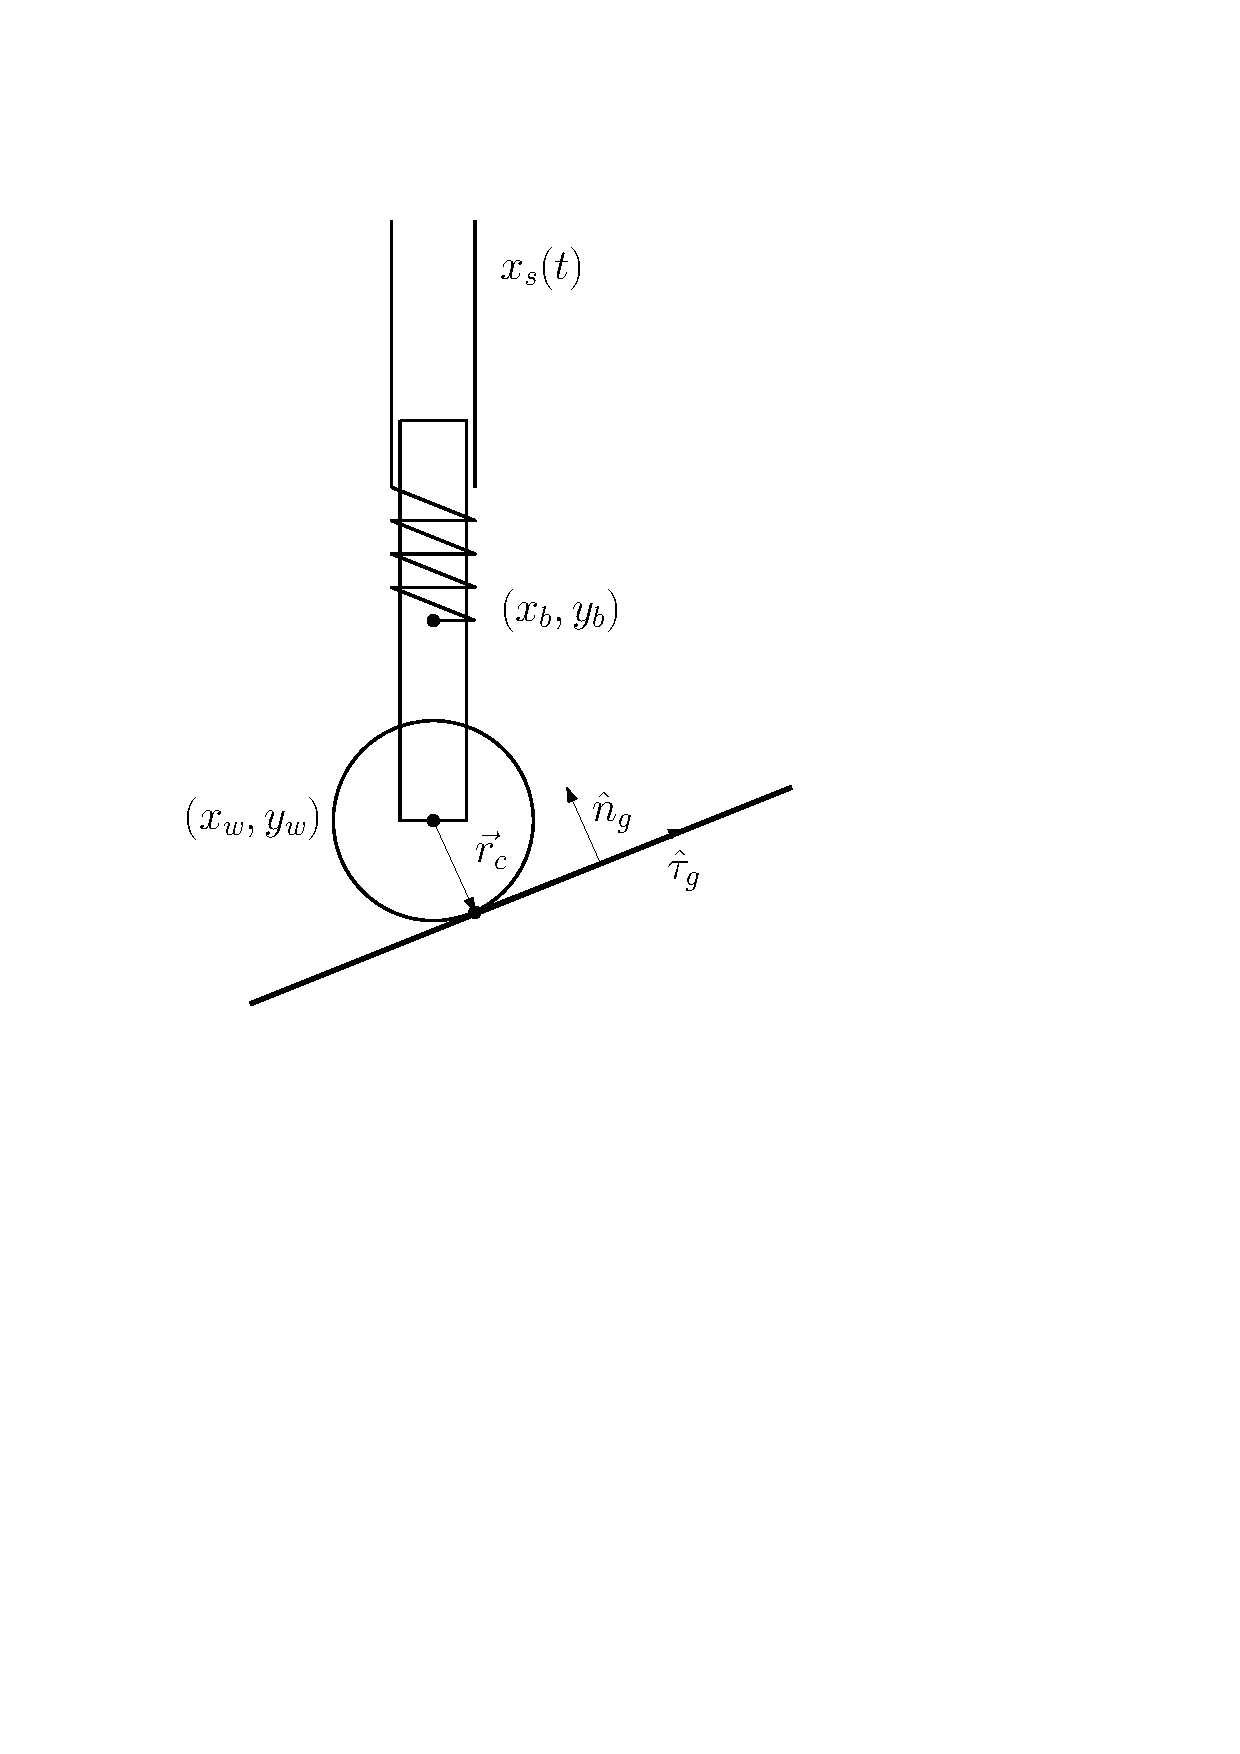
\includegraphics[scale=0.5]{diagram.pdf}
\end{center}

The velocity state vector contains the linear and angular velocities for the bar and wheel:
\[
V = 
\left[
\begin{array}{c}
u_b \\
v_b \\
\omega_b \\
u_w \\
v_w \\
\omega_w
\end{array} 
\right]
\]

The first constraint we consider is the prismatic constraint of the bar/socket system. We have that 
\[
x_b = x_s(t) \implies u_b = \dot{x}_s(t)
\]
\[
\omega_b = \omega_s = 0
\]

The second constraint is the position constraint for the wheel/bar system. 
\[
x_w - \left(x_b + \frac{L}{2}\sin \theta_b\right) = 0 \implies u_w - u_b - \frac{L}{2}\cos \theta_b \omega_b = 0
\]
\[
y_w - \left(y_b - \frac{L}{2}\cos \theta_b\right) = 0 \implies v_w - v_b - \frac{L}{2}\sin \theta_b \omega_b = 0
\]

The third constraint is the contact constraint between the wheel and ground, and is only active if the wheel and ground are in contact:
\[
(\vec{u}_w + \vec{\omega}_w \times \vec{r}_c) \cdot \hat{n}_g = 0
\]
Since the wheel is a perfect circle, the contact vector $\vec{r}_c$ is always orthogonal to the ground normal, so $(\vec{\omega}_w \times \vec{r}_c) \cdot \hat{n}_g = 0$. Since the contact impulse can only push the wheel away, we make sure that the corresponding component of $\lambda$ is greater than zero.

The final constraint is the friction constraint: 
\[
(\vec{u}_w + \vec{\omega}_w \times \vec{r}_c) \cdot \hat{\tau}_g = 0
\]
The component of $\lambda$ corresponding to this constraint is bounded by the normal impulse multiplied by the coefficient of friction, but that is ignored for simplicity.

We first solve for the constraint impulses $\lambda$ by solving the system:
\[
J V_1 = J (V_0 + M^{-1} F_{ext} \Delta t) + J M^{-1} J^T \lambda
\]
and then update the velocities:
\[
V_1 = V_0 + M^{-1} F_{ext} \Delta t + M^{-1} J^T \lambda
\]
The inverse mass matrix is 
\[
M^{-1} = 
\left[
\begin{array}{cccccc}
\frac{1}{m_b} & 0 & 0 & 0 & 0 & 0 \\
0 & \frac{1}{m_b} & 0 & 0 & 0 & 0 \\
0 & 0 & \frac{1}{I_b} & 0 & 0 & 0 \\
0 & 0 & 0 & \frac{1}{m_w} & 0 & 0 \\
0 & 0 & 0 & 0 & \frac{1}{m_w} & 0 \\
0 & 0 & 0 & 0 & 0 & \frac{1}{I_w} \\
\end{array} 
\right]
\]
The forcing vector is 
\[
F_{ext} = 
\left[
\begin{array}{c}
f_{sp,x} \\
f_{sp,y} - m_b g \\
0 \\
0 \\
-m_w g \\
0
\end{array} 
\right]
\]
All components of $JV_1$ are zero except where we have elastic collisions or a specified motion, such as that of the bar/socket system. For this constraint, we have that 
\[
JV_1^{c0} = 
\left[
\begin{array}{c}
u_s(t + \Delta t)
\end{array} 
\right]
\]
We can add Baumgarte stabilization to the bar/wheel constraint by add a term that penalizes constraint violations:
\[
JV_1^{c1} = 
\left[
\begin{array}{c}
-\beta \left[x_w - \left(x_b + \frac{L}{2}\sin \theta_b\right)\right] \\
-\beta \left[y_w - \left(y_b - \frac{L}{2}\cos \theta_b\right)\right]
\end{array} 
\right]
\]
We can also add Baumgarte stabilization to the wheel contact constraint by adding a term proportional to the penetration depth of the wheel into the ground $d_{wg}$:
\[
JV_1^{c2} = 
\left[
\begin{array}{c}
-\beta d_{wg}
\end{array} 
\right]
\]

TODO elastic collision can be handled by not setting $JV_1$ to zero

\end{document}

